% This LaTeX document needs to be compiled with XeLaTeX.
\documentclass[10pt]{article}
\usepackage[utf8]{inputenc}
\usepackage{graphicx}
\usepackage[export]{adjustbox}
\graphicspath{ {./images/} }
\usepackage{amsmath}
\usepackage{amsfonts}
\usepackage{amssymb}
\usepackage[version=4]{mhchem}
\usepackage{stmaryrd}
\usepackage{multirow}
\usepackage[fallback]{xeCJK}
\usepackage{polyglossia}
\usepackage{fontspec}
\setCJKmainfont{Noto Serif CJK JP}

\setmainlanguage{polish}
\setmainfont{CMU Serif}

\title{EGZAMIN MATURALNY Z MATEMATYKI }

\author{}
\date{}


\newcommand\Varangle{\mathop{{<\!\!\!\!\!\text{\small)}}\:}\nolimits}

\begin{document}
\maketitle
\begin{center}
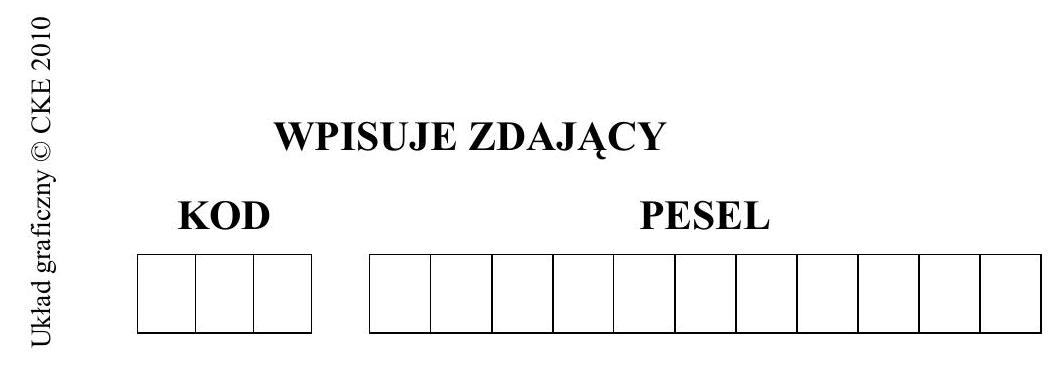
\includegraphics[max width=\textwidth]{2024_11_21_b36d8cbb94edb763da2cg-01}
\end{center}

MAJ 2011

POZIOM ROZSZERZONY

\begin{enumerate}
  \item Sprawdź, czy arkusz egzaminacyjny zawiera 19 stron (zadania 1-12). Ewentualny brak zgłoś przewodniczacemu zespołu nadzorujacego egzamin.
  \item Rozwiazzania zadań i odpowiedzi wpisuj w miejscu na to przeznaczonym.
  \item Pamiętaj, że pominięcie argumentacji lub istotnych obliczeń w rozwiązaniu zadania otwartego może spowodować, że za to rozwiązanie nie będziesz mógł dostać pełnej liczby punktów.
  \item Pisz czytelnie i używaj tylko długopisu lub pióra z czarnym tuszem lub atramentem.
  \item Nie używaj korektora, a błędne zapisy wyraźnie przekreśl.
  \item Pamiętaj, że zapisy w brudnopisie nie będą oceniane.
  \item Możesz korzystać z zestawu wzorów matematycznych, cyrkla i linijki oraz kalkulatora.
  \item Na karcie odpowiedzi wpisz swój numer PESEL i przyklej naklejkę z kodem.
  \item Nie wpisuj żadnych znaków w części przeznaczonej dla egzaminatora.
\end{enumerate}

Miejsce na naklejke z kodem

\begin{center}
\begin{tabular}{c|}
\hline
Miejsce \\
na naklejkę \\
z kodem \\
 \\
\hline
\end{tabular}
\end{center}

Czas pracy: 180 minut

Liczba punktów do uzyskania: 50

MMA-R1\_1P-112

\section*{Zadanie 1. (4 pkt)}
Uzasadnij, że dla każdej liczby całkowitej \(k\) liczba \(k^{6}-2 k^{4}+k^{2}\) jest podzielna przez 36 .\\

\includegraphics[max width=\textwidth, center]{2024_11_21_b36d8cbb94edb763da2cg-02}

\section*{Zadanie 2. (4 pkt)}
Uzasadnij, że jeżeli \(a \neq b, a \neq c, b \neq c\) i \(a+b=2 c\), to \(\frac{a}{a-c}+\frac{b}{b-c}=2\).\\

\includegraphics[max width=\textwidth, center]{2024_11_21_b36d8cbb94edb763da2cg-03}

\begin{center}
\begin{tabular}{|c|l|c|c|}
\hline
\multirow{2}{*}{\begin{tabular}{c}
Wypelnia \\
egzaminator \\
\end{tabular}} & Nr zadania & 1. & 2. \\
\cline { 2 - 4 }
 & Maks. liczba pkt & \(\mathbf{4}\) & \(\mathbf{4}\) \\
\cline { 2 - 4 }
 & Uzyskana liczba pkt &  &  \\
\hline
\end{tabular}
\end{center}

\section*{Zadanie 3. (6 pkt)}
Wyznacz wszystkie wartości parametru \(m\), dla których równanie \(x^{2}-4 m x-m^{3}+6 m^{2}+m-2=0\) ma dwa różne pierwiastki rzeczywiste \(x_{1}, x_{2}\) takie, że \(\left(x_{1}-x_{2}\right)^{2}<8(m+1)\).\\

\includegraphics[max width=\textwidth, center]{2024_11_21_b36d8cbb94edb763da2cg-04}\\

\includegraphics[max width=\textwidth, center]{2024_11_21_b36d8cbb94edb763da2cg-05}

Odpowiedź:

\begin{center}
\begin{tabular}{|c|l|c|}
\hline
\multirow{2}{*}{\begin{tabular}{c}
Wypetnia \\
egzaminator \\
\end{tabular}} & Nr zadania & 3. \\
\cline { 2 - 3 }
 & Maks. liczba pkt & 6 \\
\cline { 2 - 3 }
 & Uzyskana liczba pkt &  \\
\hline
\end{tabular}
\end{center}

\section*{Zadanie 4. (4 pkt)}
Rozwiąż równanie \(2 \sin ^{2} x-2 \sin ^{2} x \cos x=1-\cos x\) w przedziale \(\langle 0,2 \pi\rangle\).\\

\includegraphics[max width=\textwidth, center]{2024_11_21_b36d8cbb94edb763da2cg-06}

Odpowiedź:

\section*{Zadanie 5. (4 pkt)}
O ciagu ( \(x_{n}\) ) dla \(n \geq 1\) wiadomo, że:\\
a) ciagg \(\left(a_{n}\right)\) określony wzorem \(a_{n}=3^{x_{n}}\) dla \(n \geq 1\) jest geometryczny o ilorazie \(q=27\).\\
b) \(x_{1}+x_{2}+\ldots+x_{10}=145\).

Oblicz \(x_{1}\).\\

\includegraphics[max width=\textwidth, center]{2024_11_21_b36d8cbb94edb763da2cg-07}

\begin{center}
\begin{tabular}{|c|l|c|c|}
\hline
\multirow{2}{*}{\begin{tabular}{c}
Wypenia \\
egzaminator \\
\end{tabular}} & Nr zadania & \(\mathbf{4 .}\) & \(\mathbf{5 .}\) \\
\cline { 2 - 4 }
 & Maks. liczba pkt & 4 & \(\mathbf{4}\) \\
\cline { 2 - 4 }
 & Uzyskana liczba pkt &  &  \\
\hline
\end{tabular}
\end{center}

\section*{Zadanie 6. (4 pkt)}
Podstawa \(A B\) trójkąta równoramiennego \(A B C\) ma długość 8 oraz \(|\Varangle B A C|=30^{\circ}\). Oblicz długość środkowej \(A D\) tego trójkąta.\\

\includegraphics[max width=\textwidth, center]{2024_11_21_b36d8cbb94edb763da2cg-08}\\

\includegraphics[max width=\textwidth, center]{2024_11_21_b36d8cbb94edb763da2cg-09}

Odpowiedź:

\begin{center}
\begin{tabular}{|c|l|c|}
\hline
\multirow{2}{*}{\begin{tabular}{l}
Wypelnia \\
egzaminator \\
\end{tabular}} & Nr zadania & \(\mathbf{6 .}\) \\
\cline { 2 - 3 }
 & Maks. liczba pkt & \(\mathbf{4}\) \\
\cline { 2 - 3 }
 & Uzyskana liczba pkt &  \\
\hline
\end{tabular}
\end{center}

\section*{Zadanie 7. (4 pkt)}
Oblicz miarę kąta między stycznymi do okręgu \(x^{2}+y^{2}+2 x-2 y-3=0\) poprowadzonymi przez punkt \(A=(2,0)\).\\

\includegraphics[max width=\textwidth, center]{2024_11_21_b36d8cbb94edb763da2cg-10}\\

\includegraphics[max width=\textwidth, center]{2024_11_21_b36d8cbb94edb763da2cg-11}

Odpowiedź:

\begin{center}
\begin{tabular}{|c|l|c|}
\hline
\multirow{2}{*}{\begin{tabular}{l}
Wypelnia \\
egzaminator \\
\end{tabular}} & Nr zadania & 7. \\
\cline { 2 - 3 }
 & Maks. liczba pkt & 4 \\
\cline { 2 - 3 }
 & Uzyskana liczba pkt &  \\
\hline
\end{tabular}
\end{center}

\section*{Zadanie 8. (4 pkt)}
Wśród wszystkich graniastosłupów prawidłowych sześciokątnych, w których suma długości wszystkich krawędzi jest równa 24 , jest taki, który ma największe pole powierzchni bocznej. Oblicz długość krawędzi podstawy tego graniastosłupa.\\

\includegraphics[max width=\textwidth, center]{2024_11_21_b36d8cbb94edb763da2cg-12}\\

\includegraphics[max width=\textwidth, center]{2024_11_21_b36d8cbb94edb763da2cg-13}

Odpowiedź:

\begin{center}
\begin{tabular}{|c|l|c|}
\hline
\multirow{2}{*}{\begin{tabular}{l}
Wypetnia \\
egzaminator \\
\end{tabular}} & Nr zadania & 8. \\
\cline { 2 - 3 }
 & Maks. liczba pkt & 4 \\
\cline { 2 - 3 }
 & Uzyskana liczba pkt &  \\
\hline
\end{tabular}
\end{center}

\section*{Zadanie 9. (4 pkt)}
Oblicz, ile jest liczb ośmiocyfrowych, w zapisie których nie występuje zero, natomiast występują dwie dwójki i występują trzy trójki.\\

\includegraphics[max width=\textwidth, center]{2024_11_21_b36d8cbb94edb763da2cg-14}

Odpowiedź:

\section*{Zadanie 10. (3 pkt)}
Dany jest czworokąt wypukły \(A B C D\) niebędący równoległobokiem. Punkty \(M, N\) są odpowiednio środkami boków \(A B\) i \(C D\). Punkty \(P, Q\) są odpowiednio środkami przekątnych \(A C\) i \(B D\). Uzasadnij, że \(M Q \| P N\).

\begin{center}
\begin{tabular}{|c|c|c|c|c|c|c|c|c|c|c|c|c|c|c|c|c|c|c|c|c|c|c|c|c|c|c|c|}
\hline
 &  &  &  &  &  &  &  &  &  &  &  &  &  &  &  &  &  &  &  &  &  &  &  &  &  &  &  \\
\hline
 &  &  &  &  &  &  &  &  &  &  &  &  &  &  &  &  &  &  &  &  &  &  &  &  &  &  &  \\
\hline
 &  &  &  &  &  &  &  &  &  &  &  &  &  &  &  &  &  &  &  &  &  &  &  &  &  &  &  \\
\hline
 &  &  &  &  &  &  &  &  &  &  &  &  &  &  &  &  &  &  &  &  &  &  &  &  &  &  &  \\
\hline
 &  &  &  &  &  &  &  &  &  &  &  &  &  &  &  &  &  &  &  &  &  &  &  &  &  &  &  \\
\hline
 &  &  &  &  &  &  &  &  &  &  &  &  &  &  &  &  &  &  &  &  &  &  &  &  &  &  &  \\
\hline
 &  &  &  &  &  &  &  &  &  &  &  &  &  &  &  &  &  &  &  &  &  &  &  &  &  &  &  \\
\hline
 &  &  &  &  &  &  &  &  &  &  &  &  &  &  &  &  &  &  &  &  &  &  &  &  &  &  &  \\
\hline
 &  &  &  &  &  &  &  &  &  &  &  &  &  &  &  &  &  &  &  &  &  &  &  &  &  &  &  \\
\hline
 &  &  &  &  &  &  &  &  &  &  &  &  &  &  &  &  &  &  &  &  &  &  &  &  &  &  &  \\
\hline
 &  &  &  &  &  &  &  &  &  &  &  &  &  &  &  &  &  &  &  &  &  &  &  &  &  &  &  \\
\hline
 &  &  &  &  &  &  &  &  &  &  &  &  &  &  &  &  &  &  &  &  &  &  &  &  &  &  &  \\
\hline
 &  &  &  &  &  &  &  &  &  &  &  &  &  &  &  &  &  &  &  &  &  &  &  &  &  &  &  \\
\hline
 &  &  &  &  &  &  &  &  &  &  &  &  &  &  &  &  &  &  &  &  &  &  &  &  &  &  &  \\
\hline
 &  &  &  &  &  &  &  &  &  &  &  &  &  &  &  &  &  &  &  &  &  &  &  &  &  &  &  \\
\hline
 &  &  &  &  &  &  &  &  &  &  &  &  &  &  &  &  &  &  &  &  &  &  &  &  &  &  &  \\
\hline
 &  &  &  &  &  &  &  &  &  &  &  &  &  &  &  &  &  &  &  &  &  &  &  &  &  &  &  \\
\hline
 &  &  &  &  &  &  &  &  &  &  &  &  &  &  &  &  &  &  &  &  &  &  &  &  &  &  &  \\
\hline
 &  &  &  &  &  &  &  &  &  &  &  &  &  &  &  &  &  &  &  &  &  &  &  &  &  &  &  \\
\hline
 &  &  &  &  &  &  &  &  &  &  &  &  &  &  &  &  &  &  &  &  &  &  &  &  &  &  &  \\
\hline
 &  &  &  &  &  &  &  &  &  &  &  &  &  &  &  &  &  &  &  &  &  &  &  &  &  &  &  \\
\hline
 &  &  &  &  &  &  &  &  &  &  &  &  &  &  &  &  &  &  &  &  &  &  &  &  &  &  &  \\
\hline
 &  &  &  &  &  &  &  &  &  &  &  &  &  &  &  &  &  &  &  &  &  &  &  &  &  &  &  \\
\hline
 &  &  &  &  &  &  &  &  &  &  &  &  &  &  &  &  &  &  &  &  &  &  &  &  &  &  &  \\
\hline
 &  &  &  &  &  &  &  &  &  &  &  &  &  &  &  &  &  &  &  &  &  &  &  &  &  &  &  \\
\hline
 &  &  &  &  &  &  &  &  &  &  &  &  &  &  &  &  &  &  &  &  &  &  &  &  &  &  &  \\
\hline
 &  &  &  &  &  &  &  &  &  &  &  &  &  &  &  &  &  &  &  &  &  &  &  &  &  &  &  \\
\hline
 &  &  &  &  &  &  &  &  &  &  &  &  &  &  &  &  &  &  &  &  &  &  &  &  &  &  &  \\
\hline
 &  &  &  &  &  &  &  &  &  &  &  &  &  &  &  &  &  &  &  &  &  &  &  &  &  &  &  \\
\hline
 &  &  &  &  &  &  &  &  &  &  &  &  &  &  &  &  &  &  &  &  &  &  &  &  &  &  &  \\
\hline
 &  &  &  &  &  &  &  &  &  &  &  &  &  &  &  &  &  &  &  &  &  &  &  &  &  &  &  \\
\hline
 &  &  &  &  &  &  &  &  &  &  &  &  &  &  &  &  &  &  &  &  &  &  &  &  &  &  &  \\
\hline
 &  &  &  &  &  &  &  &  &  &  &  &  &  &  &  &  &  &  &  &  &  &  &  &  &  &  &  \\
\hline
 &  &  &  &  &  &  &  &  &  &  &  &  &  &  &  &  &  &  &  &  &  &  &  &  &  &  &  \\
\hline
 &  &  &  &  &  &  &  &  &  &  &  &  &  &  &  &  &  &  &  &  &  &  &  &  &  &  &  \\
\hline
 &  &  &  &  &  &  &  &  &  &  &  &  &  &  &  &  &  &  &  &  &  &  &  &  &  &  &  \\
\hline
 &  &  &  &  &  &  &  &  &  &  &  &  &  &  &  &  &  &  &  &  &  &  &  &  &  &  &  \\
\hline
 &  &  &  &  &  &  &  &  &  &  &  &  &  &  &  &  &  &  &  &  &  &  &  &  &  &  &  \\
\hline
 &  & 
\includegraphics[max width=\textwidth]{2024_11_21_b36d8cbb94edb763da2cg-15}
 &  &  &  &  &  &  &  &  &  &  &  &  &  &  &  &  &  &  &  &  &  &  &  &  &  \\
\hline
 &  &  &  &  &  &  &  &  &  &  &  &  &  &  &  &  &  &  &  &  &  &  &  &  &  &  &  \\
\hline
 &  &  &  &  &  &  &  &  &  &  &  &  &  &  &  &  &  &  &  &  &  &  &  &  &  &  &  \\
\hline
 &  &  &  &  &  &  &  &  &  &  &  &  &  &  &  &  &  &  &  &  &  &  &  &  &  &  &  \\
\hline
 &  &  &  &  &  &  &  &  &  &  &  &  &  &  &  &  &  &  &  &  &  &  &  &  &  &  &  \\
\hline
\end{tabular}
\end{center}

\begin{center}
\begin{tabular}{|c|l|c|c|}
\hline
\multirow{2}{*}{\begin{tabular}{c}
Wypelnia \\
egzaminator \\
\end{tabular}} & Nr zadania & \(\mathbf{9 .}\) & \(\mathbf{1 0 .}\) \\
\cline { 2 - 4 }
 & Maks. liczba pkt & \(\mathbf{4}\) & \(\mathbf{3}\) \\
\cline { 2 - 4 }
 & Uzyskana liczba pkt &  &  \\
\hline
\end{tabular}
\end{center}

\section*{Zadanie 11. (6 pkt)}
Dany jest ostrosłup prawidłowy czworokątny \(A B C D S\) o podstawie \(A B C D\). W trójkącie równoramiennym \(A S C\) stosunek długości podstawy do długości ramienia jest równy \(|A C|:|A S|=6: 5\). Oblicz sinus kąta nachylenia ściany bocznej do płaszczyzny podstawy.\\

\includegraphics[max width=\textwidth, center]{2024_11_21_b36d8cbb94edb763da2cg-16}\\

\includegraphics[max width=\textwidth, center]{2024_11_21_b36d8cbb94edb763da2cg-17}

Odpowiedź:

\begin{center}
\begin{tabular}{|c|l|c|}
\hline
\multirow{2}{*}{\begin{tabular}{l}
Wypełnia \\
egzaminator \\
\end{tabular}} & Nr zadania & 11. \\
\cline { 2 - 3 }
 & Maks. liczba pkt & 6 \\
\cline { 2 - 3 }
 & Uzyskana liczba pkt &  \\
\hline
\end{tabular}
\end{center}

\section*{Zadanie 12. (3 pkt)}
\(A, B\) są zdarzeniami losowymi zawartymi w \(\Omega\). Wykaż, że jeżeli \(P(A)=0,9\) i \(P(B)=0,7\), to \(P\left(A \cap B^{\prime}\right) \leq 0,3\) ( \(B^{\prime}\) oznacza zdarzenie przeciwne do zdarzenia \(B\) ).\\

\includegraphics[max width=\textwidth, center]{2024_11_21_b36d8cbb94edb763da2cg-18}

Odpowiedź:

\begin{center}
\begin{tabular}{|c|l|c|}
\hline
\multirow{2}{*}{\begin{tabular}{l}
Wypelnia \\
egzaminator \\
\end{tabular}} & Nr zadania & 12. \\
\cline { 2 - 3 }
 & Maks. liczba pkt & 3 \\
\cline { 2 - 3 }
 & Uzyskana liczba pkt &  \\
\hline
\end{tabular}
\end{center}

\section*{BRUDNOPIS}
\begin{center}
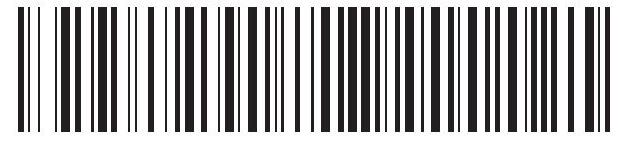
\includegraphics[max width=\textwidth]{2024_11_21_b36d8cbb94edb763da2cg-21(1)}
\end{center}

MMA-R1\_1P-112

WYPEŁNIA ZDAJĄCY

PESEL\\
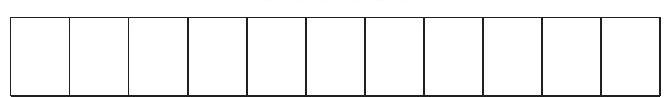
\includegraphics[max width=\textwidth, center]{2024_11_21_b36d8cbb94edb763da2cg-21}

Miejsce na naklejkę z nr PESEL

WYPEとNIA EGZAMINATOR

\begin{center}
\begin{tabular}{|c|c|c|c|c|c|c|c|}
\hline
Nr & \multicolumn{7}{|c|}{Punkty} \\
\hline
zad. & \(\mathbf{0}\) & \(\mathbf{1}\) & \(\mathbf{2}\) & \(\mathbf{3}\) & \(\mathbf{4}\) & \(\mathbf{5}\) & \(\mathbf{6}\) \\
\hline
\(\mathbf{1}\) & \(\square\) & \(\square\) & \(\square\) & \(\square\) & \(\square\) &  &  \\
\hline
\(\mathbf{2}\) & \(\square\) & \(\square\) & \(\square\) & \(\square\) & \(\square\) &  &  \\
\hline
\(\mathbf{3}\) & \(\square\) & \(\square\) & \(\square\) & \(\square\) & \(\square\) & \(\square\) & \(\square\) \\
\hline
\(\mathbf{4}\) & \(\square\) & \(\square\) & \(\square\) & \(\square\) & \(\square\) &  &  \\
\hline
\(\mathbf{5}\) & \(\square\) & \(\square\) & \(\square\) & \(\square\) & \(\square\) &  &  \\
\hline
\(\mathbf{6}\) & \(\square\) & \(\square\) & \(\square\) & \(\square\) & \(\square\) &  &  \\
\hline
\(\mathbf{7}\) & \(\square\) & \(\square\) & \(\square\) & \(\square\) & \(\square\) &  &  \\
\hline
\(\mathbf{8}\) & \(\square\) & \(\square\) & \(\square\) & \(\square\) & \(\square\) &  &  \\
\hline
\(\mathbf{9}\) & \(\square\) & \(\square\) & \(\square\) & \(\square\) & \(\square\) &  &  \\
\hline
\(\mathbf{1 0}\) & \(\square\) & \(\square\) & \(\square\) & \(\square\) &  &  &  \\
\hline
\(\mathbf{1 1}\) & \(\square\) & \(\square\) & \(\square\) & \(\square\) & \(\square\) & \(\square\) & \(\square\) \\
\hline
\(\mathbf{1 2}\) & \(\square\) & \(\square\) & \(\square\) & \(\square\) &  &  &  \\
\hline
\end{tabular}
\end{center}

\begin{center}
\begin{tabular}{|c|c|c|c|c|c|c|c|c|c|c|c|c|c|c|c|c|c|c|c|c|}
\hline
\multicolumn{21}{|l|}{\multirow[t]{4}{*}{}} \\
\hline
 &  &  &  &  &  &  &  &  &  &  &  &  &  &  &  &  &  &  &  &  \\
\hline
 &  &  &  &  &  &  &  &  &  &  &  &  &  &  &  &  &  &  &  &  \\
\hline
 &  &  &  &  &  &  &  &  &  &  &  &  &  &  &  &  &  &  &  &  \\
\hline
\end{tabular}
\end{center}

\begin{center}
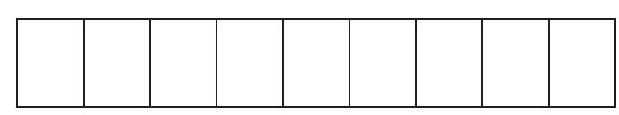
\includegraphics[max width=\textwidth]{2024_11_21_b36d8cbb94edb763da2cg-22(1)}
\end{center}

\section*{KOD EGZAMINATORA}
Czytelny podpis egzaminatora\\
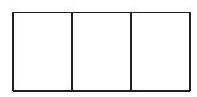
\includegraphics[max width=\textwidth, center]{2024_11_21_b36d8cbb94edb763da2cg-22}

KOD ZDAJĄCEGO


\end{document}